\section{Coding and Modulation Extensions}
\label{sec:coding}

\subsection{Baseline FEC}

The article's FEC --- reproduced bit-exactly --- is the $K=7$
convolutional code with generators $133/171/165$ (octal) at rate 1/3,
punctured to 1/2, 2/3, and 3/4, decoded by a vectorized soft-decision
Viterbi~\cite{viterbi1967}.  It remains the default and the header is
always convolutionally coded, so every extension below is backward
compatible.

\subsubsection{Encoder and Puncturing}

For input bits $u[e]$ (zero-tailed with $K-1 = 6$ flush bits), the
three coded streams are
\begin{equation}
    c_p[e] \;=\; \bigoplus_{j=0}^{6} g_p^{(j)}\, u[e-j],
    \qquad p \in \{0,1,2\},
\end{equation}
with taps $g_p$ the binary expansions of $133_8, 171_8, 165_8$.
Puncturing transmits only the positions where the rate's mask is~1
(mask column = $e \bmod P$, period $P$):
\begin{equation}
    \renewcommand{\arraystretch}{1.1}
    M_{1/2} = \begin{pmatrix} 1&1\\ 1&0\\ 0&1 \end{pmatrix},
    \qquad
    M_{2/3} = \begin{pmatrix} 1&1\\ 1&0\\ 0&0 \end{pmatrix},
    \qquad
    M_{3/4} = \begin{pmatrix} 1&1&1\\ 1&0&0\\ 0&0&0 \end{pmatrix},
\end{equation}
keeping $4/6$, $3/6$ and $4/9$ of the mother-code bits respectively.
Rate 1/3 is the all-ones mask.

\subsubsection{Soft-Decision Viterbi}

The receiver \emph{depunctures} by inserting $\lambda = 0$ (``no
opinion'') LLRs at the punctured positions --- consistent with
$L=0 \Leftrightarrow P(1)=P(0)$ --- and runs a max-log Viterbi over
the 64-state trellis.  With the sign convention of
Section~\ref{sec:llr_math}, the expected symbol for a transition from
state $s'$ with input $u$ is $x_p(s',u) \in \{-1,+1\}$
($+1 \Leftrightarrow$ coded bit 1), the branch metric is the soft
correlation
\begin{equation}
    \beta_e(s', u) \;=\; \sum_{p=0}^{2} \lambda_p[e]\; x_p(s', u),
\end{equation}
and the path metric recursion is
\begin{equation}
    \mathrm{PM}_{e+1}(s) \;=\;
    \max_{(s', u)\,\rightarrow\, s}
    \bigl[\, \mathrm{PM}_e(s') + \beta_e(s', u) \,\bigr],
\end{equation}
with the winning predecessor stored for traceback (one bit per state
per step in the C port --- the predecessor of $s$ is determined by
which of its two candidates won).  Because both $\beta$ and the LLRs
are linear in the demodulator's scale, the decoder is scale-invariant:
only the \emph{relative} weighting of carriers and bit positions
matters, which is why the front-end shape calibration of
Section~\ref{sec:llr} pays off while a global gain does not.

\subsection{LDPC}

An LDPC alternative (\texttt{ofdm\_phy/ldpc.py}) was built as an
irregular repeat--accumulate code~\cite{jin2000ira}: $N=768$, $K=256$
(rate 1/3), information-node degree 4, girth $\ge 6$, linear-time
accumulator encoding, and shortening to the payload size.  Frames carry
it via header \texttt{ver=2}, so the receiver needs no negotiation.
The construction history is itself a result: a random (4,6) matrix
\emph{lost} to the convolutional code (short cycles), and exact
sum-product decoding lost several dB end-to-end because it is
sensitive to the front end's miscalibrated LLR scale.  The shipped
decoder is normalized min-sum~\cite{chen2005minsum}
($\alpha = 0.8$ float, $\alpha = 0.75$ as $x - (x \!\gg\! 2)$ in the
integer kernel) --- deliberately, because min-sum is scale-invariant.
Measured: $+0.7$\,dB over the convolutional code on AWGN at BLER
10\,\%, compressing to $\approx$parity end-to-end at $-8$\,dB ---
the front-end LLR quality, not the code, is the binding constraint
(Section~\ref{sec:discussion}).

\subsubsection{Structure, Encoding, and Decoding}

The parity-check matrix has the IRA form
$\mathbf{H} = [\,\mathbf{H}_u \mid \mathbf{H}_{\mathrm{acc}}\,]$,
where $\mathbf{H}_u$ ($512 \times 256$, column weight 4, girth
$\ge 6$ by construction) connects information bits to checks and
$\mathbf{H}_{\mathrm{acc}}$ is the dual-diagonal accumulator.  Check
$i$ therefore reads
\begin{equation}
    \bigoplus_{v \in A(i)} u_v \;\oplus\; p_{i-1} \;\oplus\; p_i
    \;=\; 0,
\end{equation}
which gives linear-time encoding as a running XOR:
\begin{equation}
    p_i \;=\; p_{i-1} \;\oplus \bigoplus_{v \in A(i)} u_v,
    \qquad p_{-1} \equiv 0 .
\end{equation}
Shortening to a $k$-bit packet ($k \le 255$) fixes the unused
$256-k$ information positions to zero; the corresponding LLRs enter
the decoder as $+\infty$-grade priors.

Decoding is iterative normalized min-sum message passing.  With
$m_{v \to c}$ the variable-to-check and $m_{c \to v}$ the
check-to-variable messages, initialized from the channel LLRs $L_v$:
\begin{align}
    m_{c \to v} &\;=\;
        \alpha \cdot
        \Bigl( \prod_{v' \in N(c) \setminus v}
               \operatorname{sgn} m_{v' \to c} \Bigr)
        \min_{v' \in N(c) \setminus v} \bigl| m_{v' \to c} \bigr|,
        \label{eq:minsum_check}\\
    m_{v \to c} &\;=\; L_v \;+ \sum_{c' \in N(v) \setminus c}
        m_{c' \to v},
\end{align}
with hard decisions taken on the total
$L_v + \sum_{c} m_{c \to v}$ and iteration stopping early on a zero
syndrome $\mathbf{H}\hat{\mathbf{x}}^{\mathsf T} = \mathbf{0}$
(60 iterations maximum; good frames converge in a few).  The
normalization $\alpha$ compensates min-sum's overestimate of check
reliability versus exact sum--product; crucially,
Eq.~\eqref{eq:minsum_check} is homogeneous in the LLR scale, which is
why min-sum survives the front end's miscalibrated scale where exact
sum--product (whose $\tanh$ nonlinearity consumes \emph{absolute}
LLRs) measurably lost several dB.

Figure~\ref{fig:ldpc_recal} is the LDPC counterpart of the Viterbi
calibration sweep (Figure~\ref{fig:viterbi_recal}): the same raw LLRs
from each received frame are decoded four ways --- both kernels, each
on raw and on shape-mapped inputs (the exact-SPA kernel is
reconstructed for this measurement; the shipped code retains only
min-sum), 300 frames per point.  The asymmetry the equations predict
is exactly what the sweep measures.  Exact sum--product on raw LLRs
collapses $\approx$1.5--2\,dB \emph{below} min-sum (at $-9$\,dB:
0/300 versus 112/300; at $-8.5$\,dB: 19/300 versus 192/300) because
every overconfident bit in Figure~\ref{fig:llr_shape} is taken
literally by the $\tanh$ rule.  The shape map fully rescues it
(0/300 $\rightarrow$ 234/300 at $-9$\,dB), landing on par with mapped
min-sum --- once the LLRs stop lying, the exact rule has nothing left
to be hurt by.  Min-sum, meanwhile, is \emph{helped} but not gated by
the map ($\approx$1\,dB: 112/300 $\rightarrow$ 231/300 at $-9$\,dB):
its check update ignores absolute scale, but the map's cap still
defuses confidently-wrong bits in the variable-node sums, the same
mechanism as in the Viterbi path metrics.

\begin{figure}[H]
    \centering
    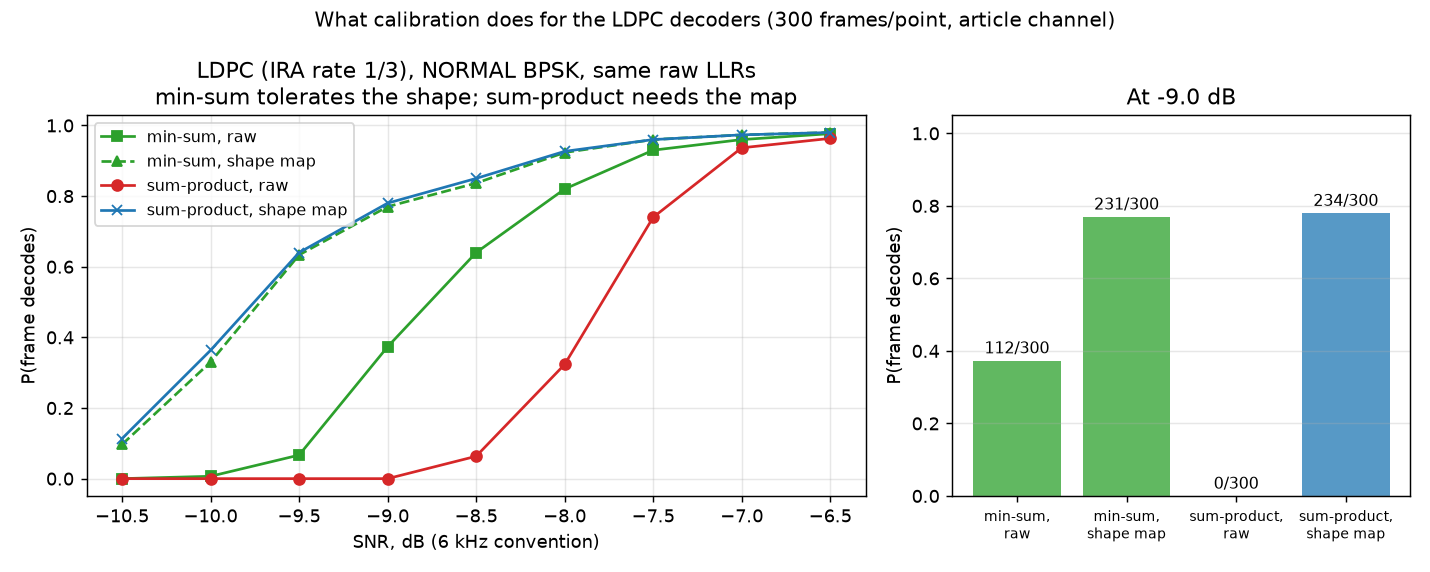
\includegraphics[width=\textwidth]{images/ldpc_recal.png}
    \caption{Calibration and the LDPC decoders (reproduce with
             \texttt{experiments/ldpc\_recal.py}; parameters and
             per-point counts in \texttt{results/ldpc\_recal.json}).
             The same received
             frames decoded by normalized min-sum and by exact
             sum--product, each from raw and from shape-mapped LLRs.
             Left: decode probability versus SNR.  Right: the four
             variants at $-9$\,dB.  Sum--product is unusable on the
             raw front end and fully recovered by the map; min-sum
             tolerates the miscalibration and still gains
             $\approx$1\,dB from it.}
    \label{fig:ldpc_recal}
\end{figure}

\subsubsection{The Code Families Head-to-Head, Calibrated}

With the front end fixed, the remaining question is which \emph{code}
is better --- the comparison that the raw front end had rendered moot
(``$\approx$parity end-to-end'').  Figure~\ref{fig:fec_comparison}
puts the fully calibrated chains side by side: convolutional +
Viterbi versus LDPC under both kernels, all on shape-mapped LLRs,
identical channel-draw sequences per variant, 300 frames per point
(binomial uncertainty $\le \pm 3$\,\% near the waterfall midpoint).
Two conclusions:

\begin{itemize}
    \item \textbf{The LDPC code gain finally materializes end-to-end:}
          $\approx$0.3--0.4\,dB at the waterfall (at $-9.5$\,dB:
          193/300 versus 151/300, i.e.\ 64\,\% versus 50\,\%; at
          $-10$\,dB: 116/300 versus 83/300).  This is consistent with
          the $+0.7$\,dB AWGN code-level measurement --- the front-end
          miscalibration was masking it, not the code failing to
          deliver it.
    \item \textbf{Calibrated min-sum $\approx$ calibrated
          sum-product:} above $-9$\,dB the two LDPC curves are
          identical to within one frame in 300.  A small exact-SPA
          edge survives only at the extreme low end (at $-10.5$\,dB:
          54/300 versus 40/300; $\approx$0.1\,dB), far below the
          rung's operating point --- so the integer min-sum kernel
          deployed in the fixed-point and C receivers gives up
          nothing measurable in the operating region.
\end{itemize}

The remaining distance to a standards-grade LDPC ($\approx$2\,dB
theoretical) is now attributable to the code construction itself
(short block, $K=256$, hand-rolled IRA), not to the decoder or the
front end --- which is precisely the open thread recorded in
Section~\ref{sec:discussion}.

\begin{figure}[H]
    \centering
    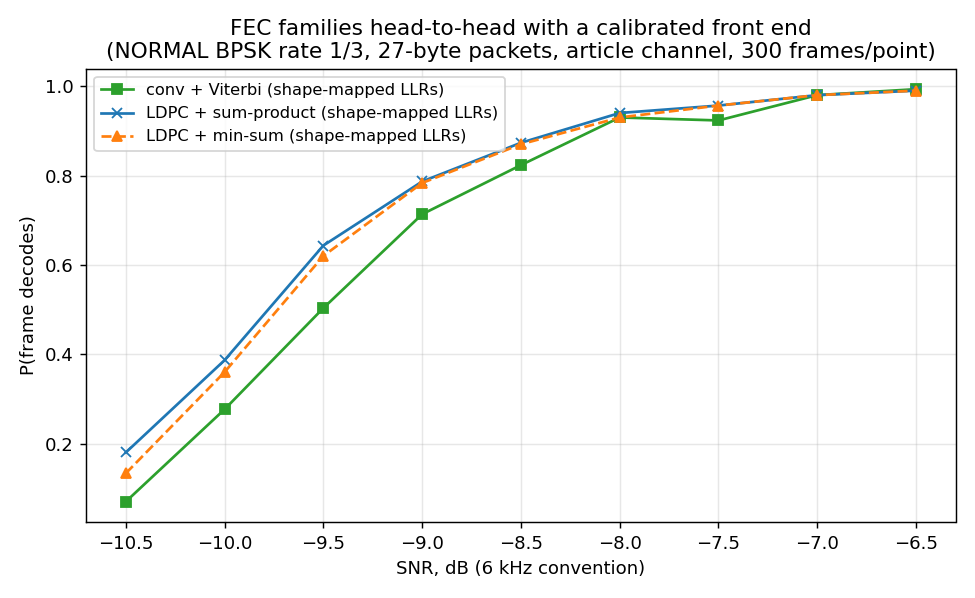
\includegraphics[width=0.8\textwidth]{images/fec_comparison.png}
    \caption{The two FEC families with a calibrated front end
             (reproduce with \texttt{experiments/fec\_comparison.py};
             every parameter and per-point count is recorded in
             \texttt{results/fec\_comparison.json}): convolutional +
             Viterbi versus LDPC with exact sum--product and with
             normalized min-sum, all decoding shape-mapped LLRs.  LDPC
             holds $\approx$0.3--0.4\,dB over the convolutional chain, and
             the two LDPC kernels are indistinguishable once
             calibrated.}
    \label{fig:fec_comparison}
\end{figure}

\subsubsection{The Same Study at the EXTREME Edge}

Figure~\ref{fig:extreme_recal} repeats the entire calibration study at
the opposite end of the ladder --- EXTREME mode ($64\times$ tiling,
BPSK rate 1/3, the $-17.9$\,dB rung-0 regime), SNR $-20.5$ to
$-16.5$\,dB, 300 frames per point, with the \emph{NORMAL-trained}
shape map applied unchanged.  Four findings:

\begin{itemize}
    \item \textbf{Scale invariance holds, as it must:} raw and
          temperature-only Viterbi decodes are bit-identical across
          all 2\,700 conv frames (asserted by the harness).
    \item \textbf{The map transfers, but only below the operating
          point.}  It buys $\approx$0.5\,dB at the deep edge (at
          $-20.5$\,dB: 138/300 versus 81/300; at $-20$\,dB: 209
          versus 157) and the gain decays to \emph{zero} by
          $-18$\,dB (279 versus 279) --- right where the rung
          actually operates.  This refines Section~\ref{sec:llr}'s
          ``accumulation-limited rungs are unaffected'': accurate at
          the operating point, where acquisition and accumulation
          dominate, but not a statement about the region below it.
    \item \textbf{Sum--product's raw-LLR penalty is far milder here}
          (at $-19.5$\,dB: 152/300 raw versus min-sum's 215, compared
          with 0/300 versus 112/300 in the NORMAL study): the
          $64\times$ coherent accumulation reshapes the LLR
          distribution and shrinks the overconfident tail the
          $\tanh$ rule chokes on.  The map still closes the gap
          completely, and calibrated min-sum and calibrated
          sum--product are again identical to the frame.
    \item \textbf{The code families reach parity at EXTREME.}  The
          calibrated head-to-head shows no consistent winner (largest
          deviation 21 frames in 300, alternating in sign) ---
          NORMAL's $\approx$0.3--0.4\,dB LDPC advantage does not
          replicate.  At the deep edge the loss budget is dominated by
          acquisition (detection failures count against every variant
          equally), so the code choice matters correspondingly less.
\end{itemize}

\begin{figure}[H]
    \centering
    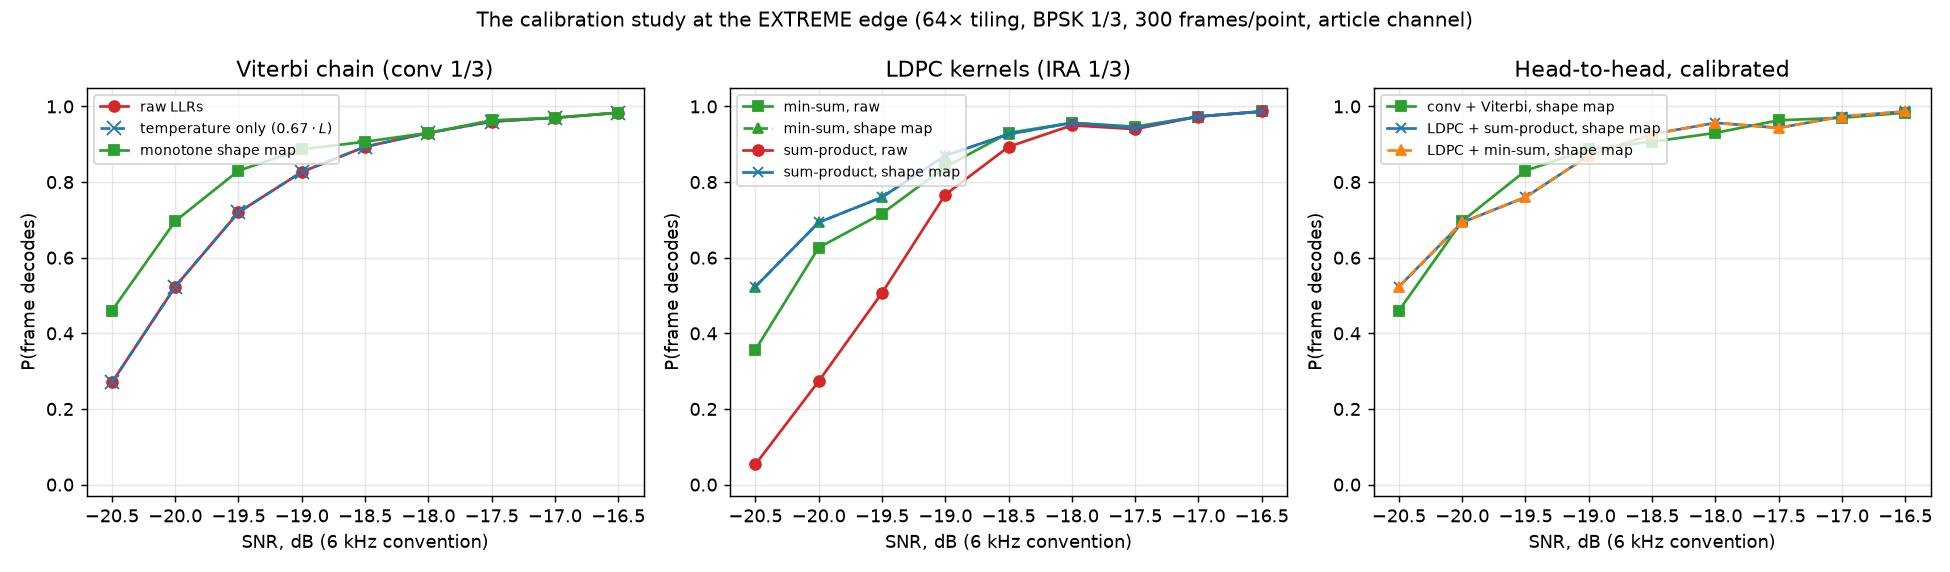
\includegraphics[width=\textwidth]{images/extreme_recal.png}
    \caption{The calibration study repeated at the EXTREME edge
             (reproduce with \texttt{experiments/extreme\_recal.py};
             parameters and per-point counts in
             \texttt{results/extreme\_recal.json}).  Left: the Viterbi
             three-way.  Middle: the LDPC kernels.  Right: the
             calibrated head-to-head --- parity, unlike
             Figure~\ref{fig:fec_comparison}'s NORMAL result.}
    \label{fig:extreme_recal}
\end{figure}

\subsubsection{\ldots{}and for 16-QAM: the Regression Is
Rate-Dependent}

Figure~\ref{fig:qam16_recal} completes the tour with 16-QAM (NORMAL
mode; rate 1/3 in the first two panels for code parity with the LDPC
code, whose only rate that is).  The result overturns the simple
version of the ``the map regresses on 16-QAM'' statement and replaces
it with a sharper one:

\begin{itemize}
    \item \textbf{At rate 1/3 the BPSK-trained map \emph{helps}
          16-QAM} by $\approx$0.4\,dB (71/300 $\rightarrow$ 109/300 at
          $-3.5$\,dB; 148 $\rightarrow$ 177 at $-3$\,dB) --- the cap's
          protection against confidently-wrong bits still pays when
          the code has redundancy to spare.
    \item \textbf{At the ladder rate (2/3) it \emph{regresses}} by
          $\approx$0.5\,dB, consistently across the waterfall
          (148/300 $\rightarrow$ 108/300 at $+1.5$\,dB; 190
          $\rightarrow$ 155 at $+2$\,dB; still 278 $\rightarrow$ 262
          at $+4$\,dB).  Under heavy puncturing each surviving bit
          carries more weight, and a correction trained on BPSK's
          single LLR class mis-weights 16-QAM's two classes (axis-sign
          versus inner/outer, Eq.~\eqref{eq:qam_llr}) faster than the
          thinner code can absorb.  The deployment gate
          ($\mu \le 2$) protects exactly the rungs that exist --- all
          ladder 16-QAM rungs are rate 1/2 and above --- so it
          remains correct, but for a rate-dependent reason, not a
          modulation-dependent one.
    \item \textbf{Calibrated min-sum \emph{beats} calibrated
          sum--product here} (215/300 versus 198/300 at $-3$\,dB;
          140 versus 115 at $-3.5$\,dB) --- the first configuration
          in these studies where the two calibrated kernels separate.
          The mechanism is the same one that sank raw-LLR SPA at
          BPSK: the BPSK-trained map leaves a \emph{residual}
          miscalibration on 16-QAM's bit classes, sum--product
          consumes it as truth, min-sum ignores it.  Min-sum is not
          merely ``as good as'' the exact rule --- it is robust to
          imperfect calibration in a way the exact rule cannot be.
    \item The code families otherwise repeat the NORMAL-BPSK pattern
          at rate 1/3: LDPC min-sum holds a small edge over
          conv+Viterbi on raw LLRs (185/300 versus 148/300 at
          $-3$\,dB, $\approx$0.2\,dB), and raw-LLR sum--product shows
          only a mild penalty (168/300) --- nothing like the BPSK
          collapse, since at these operating points the 16-QAM LLR
          distribution rarely reaches the overconfident clipped
          regime.
\end{itemize}

\begin{figure}[H]
    \centering
    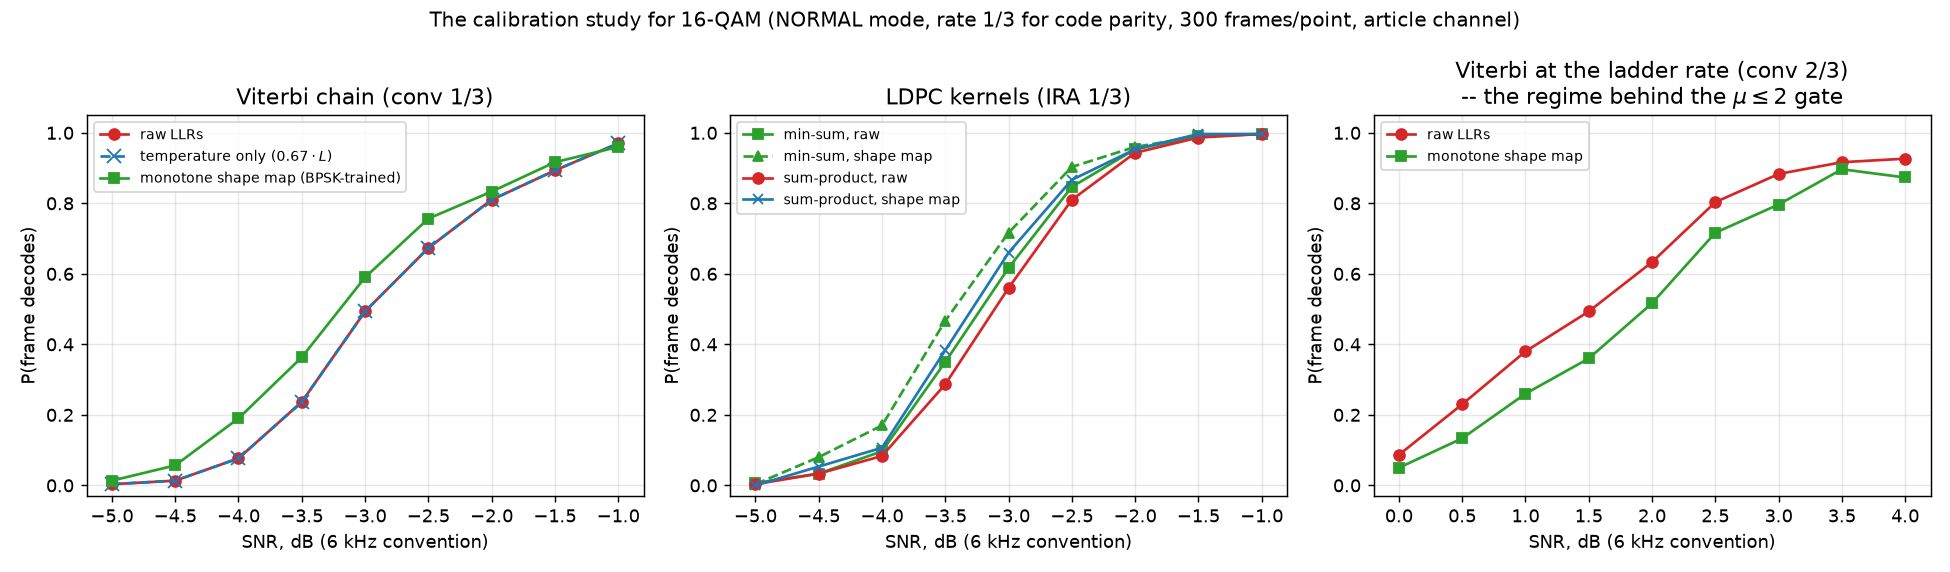
\includegraphics[width=\textwidth]{images/qam16_recal.png}
    \caption{The calibration study for 16-QAM (reproduce with
             \texttt{experiments/qam16\_recal.py}; parameters and
             per-point counts in
             \texttt{results/qam16\_recal.json}).  Left: Viterbi
             three-way at rate 1/3 --- the map \emph{helps}.  Middle:
             LDPC kernels --- calibrated min-sum beats calibrated
             sum--product for the first time.  Right: Viterbi at the
             ladder rate 2/3 --- the map \emph{regresses}, the
             measured basis of the $\mu \le 2$ deployment gate.}
    \label{fig:qam16_recal}
\end{figure}

\subsection{16-QAM}

Gray-mapped 16-QAM with max-log LLRs (separate inner/outer bit
metrics) fills the article's own ``QAM could be applied'' gap above
0\,dB, adding ladder rungs 10--12: 706\,bit/s at $+0.7$\,dB,
941\,bit/s at $+2.6$\,dB, and 1059\,bit/s at $+4.7$\,dB (PER
$\le 10\,\%$, re-measured sensitivities).
Figure~\ref{fig:qam16_const} shows received constellations across that
operating range: at $+1$\,dB the sixteen clusters are washed together
--- which is exactly why the bottom rung pairs the modulation with the
rate-1/2 code and soft LLRs rather than hard decisions --- while at
$+5$\,dB the MMSE equalizer resolves the $4\times4$ grid cleanly
enough for rate 3/4.

\begin{figure}[H]
    \centering
    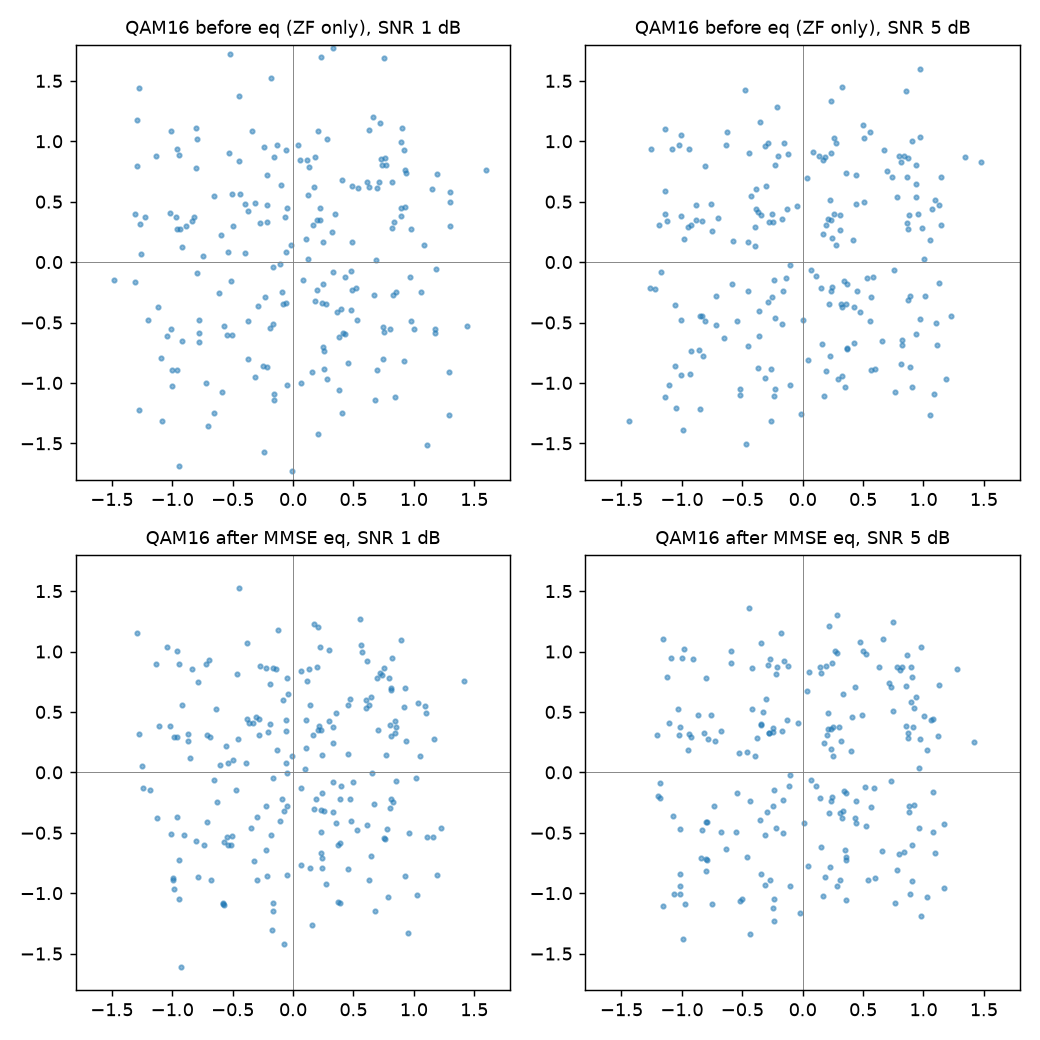
\includegraphics[width=0.78\textwidth]{images/constellation_qam16.png}
    \caption{16-QAM received constellations over the article channel
             (\texttt{experiments/figures.py}): before equalization
             (ZF pilot estimate only, top) and after Wiener-refined
             MMSE equalization (bottom), at the bottom ($+1$\,dB) and
             top ($+5$\,dB) of the 16-QAM operating range.}
    \label{fig:qam16_const}
\end{figure}

\subsection{Chase-Combining HARQ}

Because a CRC failure exports the data-block LLRs
(Section~\ref{sec:phy}), retransmissions can be soft-combined in the
Chase manner~\cite{chase1985}: the station stores the failed attempt's
LLRs, and on the next decode tries the fresh frame alone, then
fresh + stored (LLR sum), accepting whichever passes CRC
(Figure~\ref{fig:harq}).  The combining is \emph{blind} --- the ARQ
sequence number lives inside the undecodable payload, so the receiver
cannot know the retransmission is the same frame --- and \emph{safe},
because the CRC arbitrates.  Measured at $-8.5$\,dB: second-attempt
success 15/20 versus 10/20 without combining, worth $\approx$3\,dB on
a same-rung retransmission in the noise-limited regime.  Fade losses
benefit less: they are mostly synchronization-level failures that
leave no LLRs to combine.

\begin{figure}[H]
    \centering
    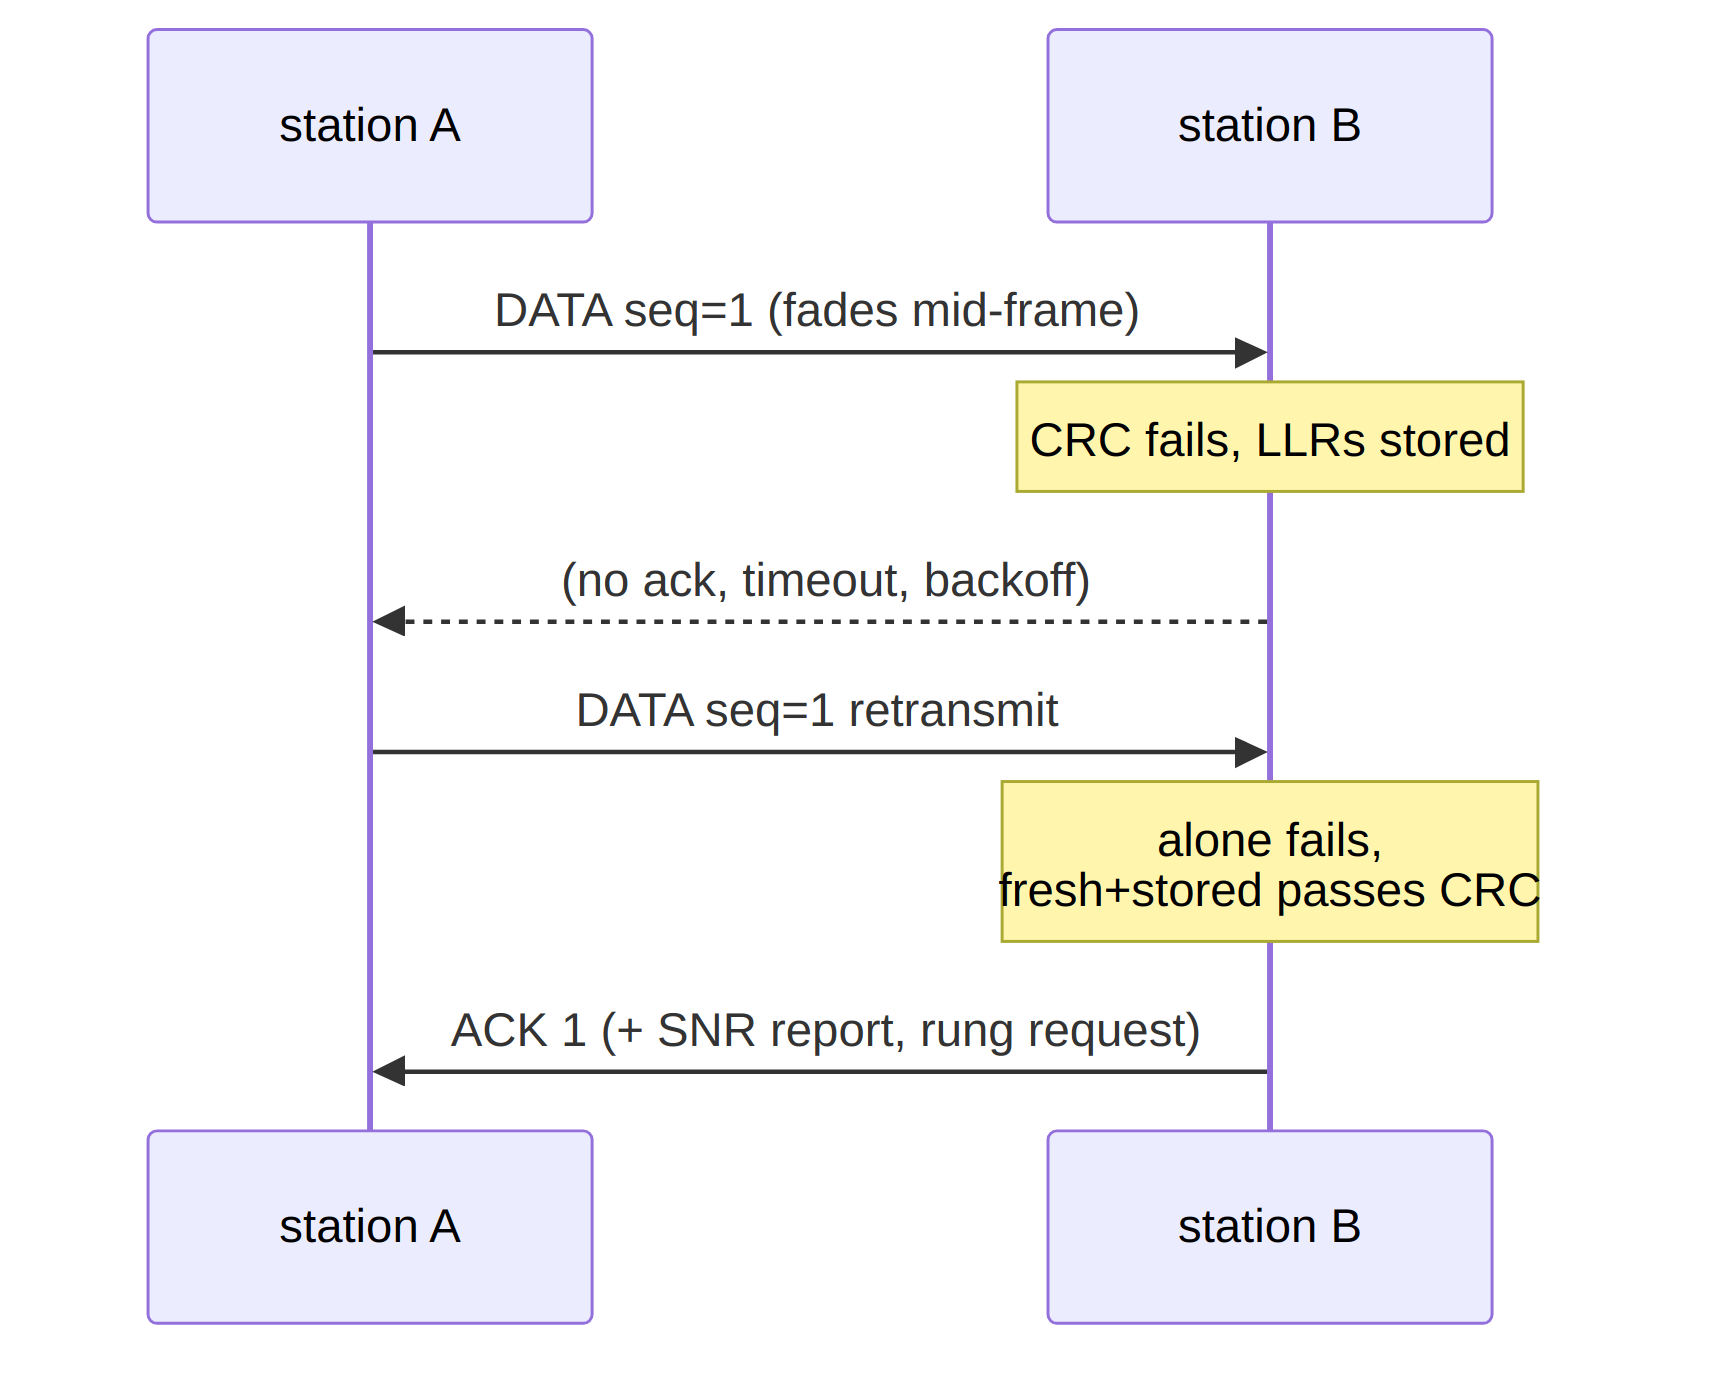
\includegraphics[width=0.8\textwidth]{images/harq_seq.png}
    \caption{Chase-combining HARQ.  No extra signalling: the stored
             LLRs come from the failed decode itself.}
    \label{fig:harq}
\end{figure}
